\chapter{Spiercontractie en motoriek}\label{ch:b2:muscle-movement}

Een sprintster verlaat de startblokken met een kracht op de baan van drie
keer haar gewicht, ontwikkeld in een vijfde van een seconde door spieren die
een ogenblik eerder slap waren. Niets in de cel werd daarvoor korter: de
filamenten binnenin gleden langs elkaar, getrokken door miljoenen moleculaire
handen die elk een stap van tien nanometer zetten en loslaten, tien keer per
seconde, betaald met één ATP per keer. Dit hoofdstuk neemt de \omterm{def:b2:cell-differentiation:myogenesis}{spiervezel} die
in \cref{ch:b2:cell-differentiation} werd gebouwd en laat haar werken: het
glijden van de filamenten en de motor die ze aandrijft, de calciumschakelaar
die de motor aan- en uitzet, het bevel van de zenuw, de mechanica van kracht
en snelheid, en de manier waarop het zenuwstelsel het geheel doseert, van een
enkele samentrekking tot een sprint.

\section{De glijdende filamenten}

\begin{proposition}[Het mechanisme van de glijdende filamenten]\label{prop:b2:muscle-movement:sliding}
\index{glijdend filament}\index{sarcomeer!contractie}
Wanneer een \omterm{def:b2:cell-differentiation:myogenesis}{spiervezel} korter wordt, worden haar sarcomeren korter
(\cref{ch:b2:cell-differentiation}), maar noch de dikke filamenten van
myosine noch de dunne filamenten van actine veranderen van lengte: de dunne
filamenten glijden naar binnen langs de dikke, de I-band en de H-zone worden
smaller, en de Z-schijven naderen elkaar. De overlap tussen de twee sets
filamenten is waar kracht wordt opgewekt, en een \omterm{def:b2:cell-differentiation:fibre}{sarcomeer} levert kracht
in verhouding tot de overlap: vanaf een uitgerekte lengte van
\qty{3.6}{\micro m}, zonder overlap en zonder kracht, stijgt de kracht
lineair naarmate de filamenten meer overlappen, bereikt een plateau rond
\qty{2.2}{\micro m}, waar elke myosinekop tegenover actine ligt, en daalt
weer onder \qty{2.0}{\micro m}, wanneer de dunne filamenten tegen elkaar
botsen en de dikke tegen de Z-schijven stoten. De rustlengte van een spier
in het lichaam ligt op het plateau --- de eerste aanwijzing voor hoe de
kracht wordt gemaakt.
\end{proposition}
\begin{proof}[Bewijsmateriaal]
A.~F.~Huxley en Niedergerke, en H.~E.~Huxley en Hanson (1954), maten met
interferentie- en fasecontrastmicroscopie de banden van afzonderlijke vezels
en van geïsoleerde myofibrillen terwijl die korter werden: de A-band behield
zijn lengte, de I-band kromp, dus de filamenten glijden. Gordon, Huxley en
Julian (1966) hielden een enkele vezel op vaste lengtes met een
terugkoppelingsapparaat dat de sarcomeerlengte van één segment constant hield,
en vonden dat de kracht evenredig was met de overlap van dikke en dunne
filamenten, gemeten met elektronenmicroscopie --- de lengte-spanningscurve
met haar plateau en twee lineaire takken, precies zoals de geometrie van de
filamenten voorspelt.
\end{proof}

\begin{omfigure}
\begin{minipage}[b]{0.5\linewidth}\centering
\begin{tikzpicture}[every node/.style={font=\scriptsize}]
  \foreach \y/\lab/\ov in {2.4/{ontspannen, \qty{2.6}{\micro m}}/0.9, 1.2/{verkort, \qty{2.0}{\micro m}}/0.3} {
    \begin{scope}[yshift=\y cm]
      \draw[very thick, omThm] (0,-0.35) -- (0,0.35); \draw[very thick, omThm] (4.4-2*\ov+1.0,-0.35) -- (4.4-2*\ov+1.0,0.35);
      \pgfmathsetmacro{\len}{4.4-2*\ov+1.0}
      \foreach \dy in {-0.25,0.05,0.25} { \draw[thick, omDef] (0,\dy) -- (1.5,\dy); \draw[thick, omDef] (\len,\dy) -- (\len-1.5,\dy); }
      \draw[line width=3pt, omExo!80!black] (\len/2-1.1,-0.1) -- (\len/2+1.1,-0.1);
      \node[right] at (\len+0.15,0) {\lab};
    \end{scope}
  }
  \node[align=center] at (2.7,0.1) {de filamenten behouden hun lengte;\\de overlap groeit terwijl\\de Z-schijven naderen};
\end{tikzpicture}
\end{minipage}\hfill
\begin{minipage}[b]{0.48\linewidth}\centering
\begin{tikzpicture}
\begin{axis}[
  width=\linewidth, height=4.8cm,
  axis x line=bottom, axis y line=left,
  xmin=1.2, xmax=3.8, ymin=0, ymax=1.15,
  xlabel={sarcomeerlengte (\unit{\micro m})}, ylabel={kracht (relatief)},
  xlabel style={font=\scriptsize, at={(axis description cs:0.5,-0.17)}, anchor=north},
  ylabel style={font=\scriptsize},
  tick label style={font=\scriptsize}, xtick={1.3,2.0,2.2,3.6}, ytick={0,0.5,1},
  clip=false,
]
\addplot[very thick, omDef] coordinates {(1.3,0) (1.65,0.5) (2.0,1) (2.2,1) (3.6,0)};
\node[font=\scriptsize, anchor=south] at (axis cs:2.1,1.02) {plateau};
\node[font=\scriptsize, anchor=west, align=left] at (axis cs:2.95,0.75) {afnemende\\overlap};
\end{axis}
\end{tikzpicture}
\end{minipage}

{\small Links: een \omterm{def:b2:cell-differentiation:fibre}{sarcomeer} ontspannen en samengetrokken --- de dunne
filamenten (blauw) glijden langs de dikke (grijs) zonder van lengte te
veranderen. Rechts: de lengte-spanningscurve: de kracht is evenredig met de
overlap, maximaal op het plateau waar de spier in rust ligt.}
\end{omfigure}

\begin{omfigure}
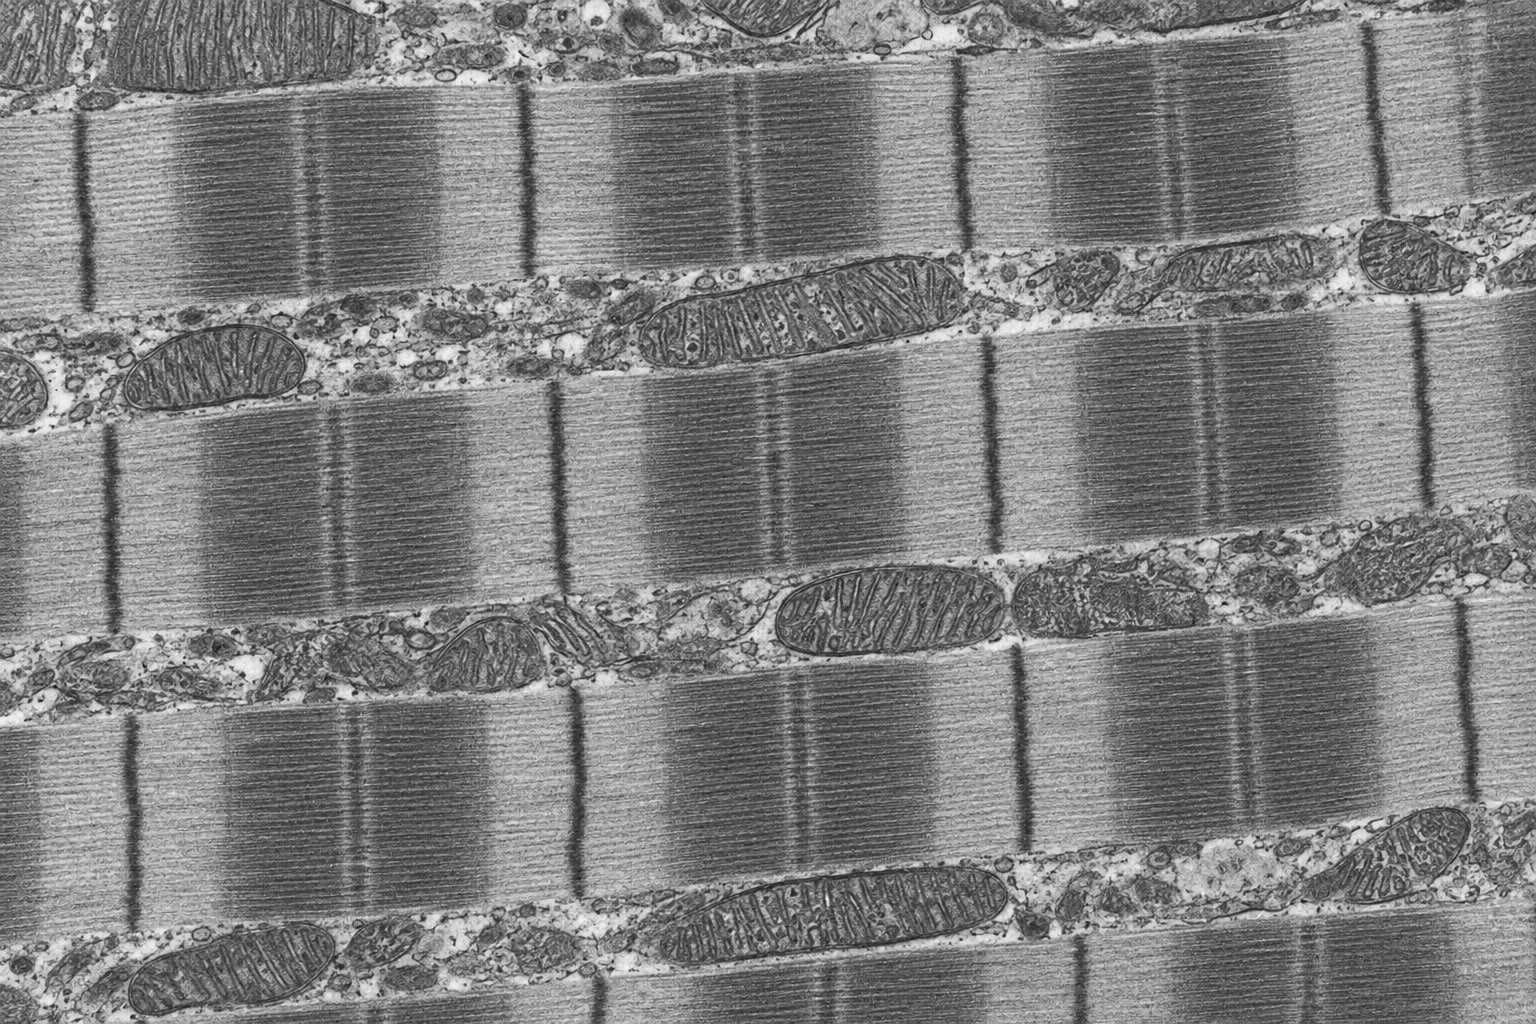
\includegraphics[width=0.6\linewidth]{images/book4/ai/b4-21-sarcomere-tem.jpg}

{\small Myofibrillen onder de elektronenmicroscoop: de A-banden van dikke
filamenten, de I-banden van dunne filamenten, doorsneden door Z-lijnen, en de
mitochondriën tussen de fibrillen die het glijden betalen.}
\end{omfigure}

\section{De motor}

\begin{proposition}[De dwarsbruggencyclus]\label{prop:b2:muscle-movement:crossbridge}
\index{dwarsbruggencyclus}\index{myosine}\index{ATP!bij contractie}
Elk dik filament zit vol met zo'n driehonderd \emph{myosinekoppen}, en elke
kop is een motor die in een cyclus van vier stappen langs actine loopt. (1)
Met ATP gebonden is de kop los van actine; hij hydrolyseert het ATP tot ADP en
fosfaat en spant zich in een gespannen vorm met hoge energie. (2) De gespannen
kop bindt een actinesubeenheid en vormt een \emph{dwarsbrug}. (3) Het fosfaat
komt vrij en de kop klapt terug naar zijn ontspannen vorm, waarbij hij het
dunne filament zo'n \qty{10}{nm} naar het midden van het \omterm{def:b2:cell-differentiation:fibre}{sarcomeer} trekt ---
de \emph{krachtslag}; ADP verlaat de kop. (4) Een nieuw ATP bindt en de kop
laat de actine los; zonder ATP kan hij niet loslaten, en dat is de
lijkstijfheid. De cyclus duurt ongeveer een twintigste van een seconde; een
kop is het grootste deel ervan los, zodat op elk ogenblik slechts een fractie
van de koppen trekt en een filament dat snel glijdt nooit wordt losgelaten.
De kracht is de som van de trekken van de gebonden koppen; de verkorting is
de optelsom van hun stappen, hoogstens een halve micrometer per \omterm{def:b2:cell-differentiation:fibre}{sarcomeer} per
cyclus; en de energie is één ATP per stap per kop, ongeveer
\qty{50}{kJ/mol} --- \qty{8e-20}{J} per stap, waarvan de kop tot de helft in
arbeid omzet.
\end{proposition}

\begin{omfigure}
\begin{tikzpicture}[every node/.style={font=\scriptsize}, >=stealth]
  \foreach \x/\lab/\ang/\att in {0/{1. ATP gebonden:\\los; ATP\\gehydrolyseerd, kop gespannen}/60/0, 3.6/{2. gespannen kop\\bindt actine:\\dwarsbrug}/60/1, 7.2/{3. fosfaat vrij:\\krachtslag,\\filament \qty{10}{nm} verschoven}/20/1, 10.8/{4. ADP weg, nieuw\\ATP bindt: kop\\laat los}/20/0} {
    \begin{scope}[xshift=\x cm]
      \draw[thick, omDef] (0,2.2) -- (2.8,2.2); \foreach \i in {0.2,0.6,...,2.6} \fill[omDef!50] (\i,2.2) circle (0.14);
      \draw[line width=3pt, omExo!80!black] (0,0.4) -- (2.8,0.4);
      \draw[very thick, omThm] (1.4,0.4) -- (1.4,1.0);
      \ifnum\att=1 \draw[very thick, omThm] (1.4,1.0) -- ++(\ang:1.15); \fill[omThm] (1.4,1.0) ++(\ang:1.15) circle (0.16); \else \draw[very thick, omThm] (1.4,1.0) -- ++(\ang:1.0); \fill[omThm] (1.4,1.0) ++(\ang:1.0) circle (0.16); \fi
      \node[below, align=center] at (1.4,0.15) {\lab};
    \end{scope}
  }
  \draw[->, thick, omDef] (7.9,2.55) -- (8.9,2.55); \node[omDef, above] at (8.4,2.6) {dun filament beweegt};
\end{tikzpicture}

{\small De \omterm{prop:b2:muscle-movement:crossbridge}{dwarsbruggencyclus}. Een gespannen myosinekop (rood) bindt actine
(blauw), laat fosfaat vrij en trekt met zijn krachtslag aan het dunne
filament, bindt daarna een vers ATP en laat los.}
\end{omfigure}

\begin{theorem}[Kracht, snelheid en vermogen van een spier]\label{thm:b2:muscle-movement:hill}
\index{kracht-snelheidscurve}\index{spiervermogen}
De kracht van een spier daalt naarmate ze sneller verkort, omdat hoe sneller
de filamenten glijden, hoe minder koppen er op elk ogenblik gebonden zijn en
hoe meer ervan voorbij hun slag worden meegesleept voordat ze loslaten. De
relatie van Hill beschrijft dit:
\[
(F + a)(v + b) = (F_0 + a)\,b,
\]
waarin $F_0$ de isometrische kracht is (bij $v = 0$), $v_{\max} =
F_0 b/a$ de snelheid zonder belasting, en $a$, $b$ constanten ($a \approx
F_0/4$). Het vermogen $Fv$ is nul aan beide uiteinden en het grootst bij
ongeveer een derde van $v_{\max}$ en een derde van $F_0$ --- daarom schakelt
een wielrenner en heeft de pas van een sprinter een voorkeursritme. Een
menselijke spier ontwikkelt ongeveer \qty{30}{N} per vierkante centimeter
doorsnede, verkort met tot tien lengtes per seconde, en levert op haar best
zo'n \qty{100}{W} per kilogram.
\end{theorem}
\begin{proof}
De curve van Hill is empirisch (1938), gemeten op een geïsoleerde
kikkerspier als de verkortingssnelheid tegen de last die ze optilt; de
hyperbool past omdat de fractie gebonden koppen daalt met de glijsnelheid en
de kracht van elke gebonden kop daalt terwijl hij door zijn slag wordt
meegevoerd. Vermogen: met $F = (F_0 + a)b/(v + b) - a$ is $Fv$ nul bij
$v = 0$ en bij $v_{\max}$; differentiëren geeft het maximum bij
$v = b(\sqrt{(F_0 + a)/a} - 1)$, wat voor $a = F_0/4$ neerkomt op $v =
1.24\,b = 0.31\,v_{\max}$, waar $F = 0.31\,F_0$.
\end{proof}

\begin{omfigure}
\begin{tikzpicture}
\begin{axis}[
  width=0.7\linewidth, height=5.4cm,
  axis x line=bottom, axis y line=left,
  xmin=0, xmax=1.05, ymin=0, ymax=1.1,
  xlabel={verkortingssnelheid $v/v_{\max}$}, ylabel={kracht $F/F_0$, vermogen (relatief)},
  xlabel style={font=\small, at={(axis description cs:0.5,-0.13)}, anchor=north},
  ylabel style={font=\small},
  tick label style={font=\small}, xtick={0,0.31,1}, xticklabels={0,0.31,1}, ytick={0,0.31,1}, yticklabels={0,0.31,1},
  legend style={font=\scriptsize, at={(0.97,0.95)}, anchor=north east, draw=none},
  clip=false,
]
\addplot[very thick, omDef, domain=0:1, samples=100] {(1.25*0.25)/(x+0.25) - 0.25};
\addlegendentry{kracht}
\addplot[very thick, omThm, domain=0:1, samples=100] {10.4*x*((1.25*0.25)/(x+0.25) - 0.25)};
\addlegendentry{vermogen (geschaald)}
\draw[dashed, gray] (axis cs:0.31,0) -- (axis cs:0.31,1.0);
\end{axis}
\end{tikzpicture}

{\small De \omterm{thm:b2:muscle-movement:hill}{kracht-snelheidscurve} van Hill ($a = F_0/4$) en het vermogen dat
eruit volgt: de kracht daalt naarmate de spier sneller verkort, en het
vermogen piekt bij ongeveer een derde van de maximale snelheid en een derde
van de isometrische kracht.}
\end{omfigure}

\section{De schakelaar: calcium}

\begin{proposition}[Excitatie-contractiekoppeling]\label{prop:b2:muscle-movement:coupling}
\index{excitatie-contractiekoppeling}\index{troponine}\index{tropomyosine}\index{sarcoplasmatisch reticulum}
In rust kunnen de myosinekoppen de actine niet bereiken: de bindingsplaatsen
op het dunne filament zijn bedekt door \emph{tropomyosine}, een staaf die in
de groef van de actinehelix ligt en daar door \emph{troponine} wordt
vastgehouden. De schakelaar is calcium. Een actiepotentiaal op het membraan
van de vezel loopt via de T-tubuli naar binnen en opent, op de verbindingen
waar een \omterm{def:b2:cell-differentiation:fibre}{T-tubulus} het \omterm{def:b2:cell-differentiation:fibre}{sarcoplasmatisch reticulum} raakt, de
calciumafgiftekanalen van het reticulum; calcium overspoelt de myofibrillen,
stijgt in een milliseconde van \qty{0.1}{} tot \qty{10}{\micro mol/L},
bindt troponine, en troponine schuift tropomyosine van de bindingsplaatsen:
de koppen hechten zich, en de vezel trekt samen zolang het calcium blijft.
Pompen in het reticulum, die ATP verbruiken, halen het calcium binnen enkele
tientallen milliseconden terug; tropomyosine bedekt de plaatsen opnieuw en de
vezel ontspant. Ontspanning is dus even actief als samentrekking, en een spier
zonder ATP kan haar koppen niet loslaten en haar calcium niet wegpompen ---
rigor mortis. In het \omterm{def:b2:heart:anatomy}{hart} wordt dezelfde schakelaar gebruikt, maar met
calcium dat van buiten via de eigen kanalen van het membraan binnenkomt om de
afgifte in gang te zetten, en daarom is het \omterm{def:b2:heart:anatomy}{hart}, en niet de skeletspier,
gevoelig voor het calcium in het \omterm{def:b2:blood-circulation:blood}{bloed}.
\end{proposition}

\begin{omfigure}
\begin{tikzpicture}[every node/.style={font=\scriptsize}, >=stealth]
  \node[draw, rounded corners, fill=omDef!15, align=center] (nerve) at (0,0) {impuls in de\\motorische zenuw};
  \node[draw, rounded corners, fill=omDef!15, align=center] (nmj) at (3.0,0) {neuromusculaire\\overgang:\\acetylcholine};
  \node[draw, rounded corners, fill=omDef!15, align=center] (ap) at (6.2,0) {actiepotentiaal\\van de spier, via\\de T-tubuli};
  \node[draw, rounded corners, fill=omThm!15, align=center] (ca) at (9.4,0) {Ca$^{2+}$ vrijgegeven\\uit het sarcoplasmatisch\\reticulum};
  \node[draw, rounded corners, fill=omProp!20, align=center] (tn) at (12.6,0) {troponine bindt Ca$^{2+}$,\\tropomyosine verschuift,\\koppen hechten zich};
  \node[draw, rounded corners, fill=omExo!25, align=center] (off) at (9.4,-2.2) {pompen halen Ca$^{2+}$ terug (ATP);\\tropomyosine bedekt actine:\\ontspanning};
  \draw[->, thick] (nerve) -- (nmj); \draw[->, thick] (nmj) -- (ap); \draw[->, thick] (ap) -- (ca); \draw[->, thick] (ca) -- (tn);
  \draw[->, thick] (ca) -- (off);
  \node[below, gray] at (1.5,-0.7) {\qty{0.6}{ms}}; \node[below, gray] at (4.6,-0.7) {\qty{1}{ms}}; \node[below, gray] at (7.8,-0.7) {\qty{1}{ms}};
\end{tikzpicture}

{\small Van zenuwimpuls tot kracht: de overgang, de eigen actiepotentiaal van
de vezel, de afgifte van calcium en het vrijmaken van de actineplaatsen ---
en daarna de pompen die er een eind aan maken.}
\end{omfigure}

\section{Bevel en dosering}

\begin{definition}[De motorische eenheid]\label{def:b2:muscle-movement:motorunit}
\index{motorische eenheid}\index{enkelvoudige contractie}\index{tetanus}\index{rekrutering}
Een \emph{motorisch \omterm{def:b2:neurons-synapses:neuron}{neuron}} in het ruggenmerg stuurt zijn \omterm{def:b2:neurons-synapses:neuron}{axon} naar een spier
en vertakt zich om van een handvol tot duizend vezels te innerveren, verspreid
door de spier; het \omterm{def:b2:neurons-synapses:neuron}{neuron} en zijn vezels vormen een \emph{motorische
eenheid}, de kleinste hoeveelheid kracht die het zenuwstelsel kan bevelen.
Elke impuls in het \omterm{def:b2:neurons-synapses:neuron}{neuron} laat elke vezel van de eenheid één keer vuren en
een \emph{enkelvoudige contractie} geven: een kracht die in zo'n \qty{30}{ms}
stijgt en in \qty{100}{ms} afneemt, omdat de calciumpuls kort is. Impulsen
die snel op elkaar volgen, laten de contracties optellen, omdat het calcium
van de ene nog niet is weggepompt wanneer de volgende aankomt; bij zo'n 30
tot 50 impulsen per seconde versmelt de kracht tot een gladde
\emph{tetanus}, drie tot vijf keer de enkelvoudige contractie. Het
zenuwstelsel doseert de kracht van een spier op twee manieren: met de
\emph{frequentie} waarmee elke eenheid vuurt, en met het \emph{aantal}
eenheden dat het rekruteert --- eerst kleine, trage, vermoeiingsbestendige
eenheden (het \emph{grootteprincipe}), en als laatste grote, snelle, alleen
voor de grootste inspanningen. Een spier in gewoon gebruik staat dus nooit
volledig aan: een fractie van haar eenheden vuurt, bij toerbeurt, en de rest
rust.
\end{definition}

\begin{omfigure}
\begin{tikzpicture}
\begin{axis}[
  width=0.82\linewidth, height=5.4cm,
  axis x line=bottom, axis y line=left,
  xmin=0, xmax=1.0, ymin=0, ymax=4.2,
  xlabel={tijd (s)}, ylabel={kracht (enkelvoudige contractie $=$ 1)},
  xlabel style={font=\small, at={(axis description cs:0.5,-0.13)}, anchor=north},
  ylabel style={font=\small},
  tick label style={font=\small}, xtick={0,0.2,0.4,0.6,0.8,1}, ytick={0,1,2,3,4},
  clip=false,
]
% single twitch
\addplot[very thick, omDef, domain=0:0.2, samples=60] {(x<0.02)*0 + (x>=0.02)*4.5*(x-0.02)*exp(-(x-0.02)/0.03)*4.1};
% summation at 10 Hz
\addplot[very thick, omProp, domain=0.25:0.62, samples=200] {(x>=0.25)*4.5*4.1*(x-0.25)*exp(-(x-0.25)/0.03) + (x>=0.33)*4.5*4.1*(x-0.33)*exp(-(x-0.33)/0.03) + (x>=0.41)*4.5*4.1*(x-0.41)*exp(-(x-0.41)/0.03) + (x>=0.49)*4.5*4.1*(x-0.49)*exp(-(x-0.49)/0.03)};
% tetanus at 50 Hz
\addplot[very thick, omThm, domain=0.66:0.98, samples=100] {3.8*(1-exp(-(x-0.66)/0.06))};
\node[font=\scriptsize, anchor=west] at (axis cs:0.09,0.7) {één impuls: enkelvoudige contractie};
\node[font=\scriptsize, anchor=south] at (axis cs:0.44,2.2) {\qty{12}{Hz}: summatie};
\node[font=\scriptsize, anchor=south] at (axis cs:0.82,3.85) {\qty{50}{Hz}: gefuseerde tetanus};
\end{axis}
\end{tikzpicture}

{\small Kracht doseren met de frequentie. Eén impuls geeft een \omterm{def:b2:muscle-movement:motorunit}{enkelvoudige
contractie}; impulsen met een twaalftal per seconde tellen op tot een golvende
kracht; bij vijftig per seconde versmelt de kracht tot een \omterm{def:b2:muscle-movement:motorunit}{tetanus} die
meerdere keren de \omterm{def:b2:muscle-movement:motorunit}{enkelvoudige contractie} bedraagt.}
\end{omfigure}

\begin{proposition}[Reflexen en het ruggenmerg]\label{prop:b2:muscle-movement:reflex}
\index{reflexboog}\index{spierspoeltje}\index{rekreflex}\index{reciproke remming}
Het motorische \omterm{def:b2:neurons-synapses:neuron}{neuron} is de \emph{gemeenschappelijke eindweg}: elk bevel, uit
de cortex of uit een reflex, eindigt erop. Het eenvoudigste circuit is de
\emph{rekreflex} van \cref{ch:b2:neurons-synapses}: sensorische uiteinden die
om speciale vezels binnen in de spier zijn gewonden, de
\emph{spierspoeltjes}, vuren wanneer de spier wordt uitgerekt, prikkelen via
één \omterm{def:b2:neurons-synapses:synapse}{synaps} de motorische \omterm{def:b2:neurons-synapses:neuron}{neuronen} van dezelfde spier, en remmen via een
schakelneuron die van de antagonist (\emph{\omterm{prop:b2:muscle-movement:reflex}{reciproke remming}}), zodat de
spier zich tegen de rekking verzet --- de basis van de houding, omdat elke
zwaai een rekking van een of andere spier is. Een tweede receptor, het
peeslichaampje, vuurt wanneer de kracht van de spier hoog is en remt de eigen
motorische \omterm{def:b2:neurons-synapses:neuron}{neuronen}: een veiligheidsklep. Terugtrekken van een pijnlijke
prikkel is een reflex van meerdere synapsen die het ledemaat buigt en aan de
andere kant het andere strekt, zodat men niet valt. En de hersenen bevelen
geen spieren maar bewegingen: de cortex stuurt een plan, de kleine hersenen
corrigeren het met wat de spierspoeltjes melden, de basale ganglia geven het
vrij, en de circuits van het ruggenmerg, die op eigen kracht een stapritme
kunnen onderhouden, voeren het uit --- het onderwerp van het deel van jaar 3.
\end{proposition}

\begin{omfigure}
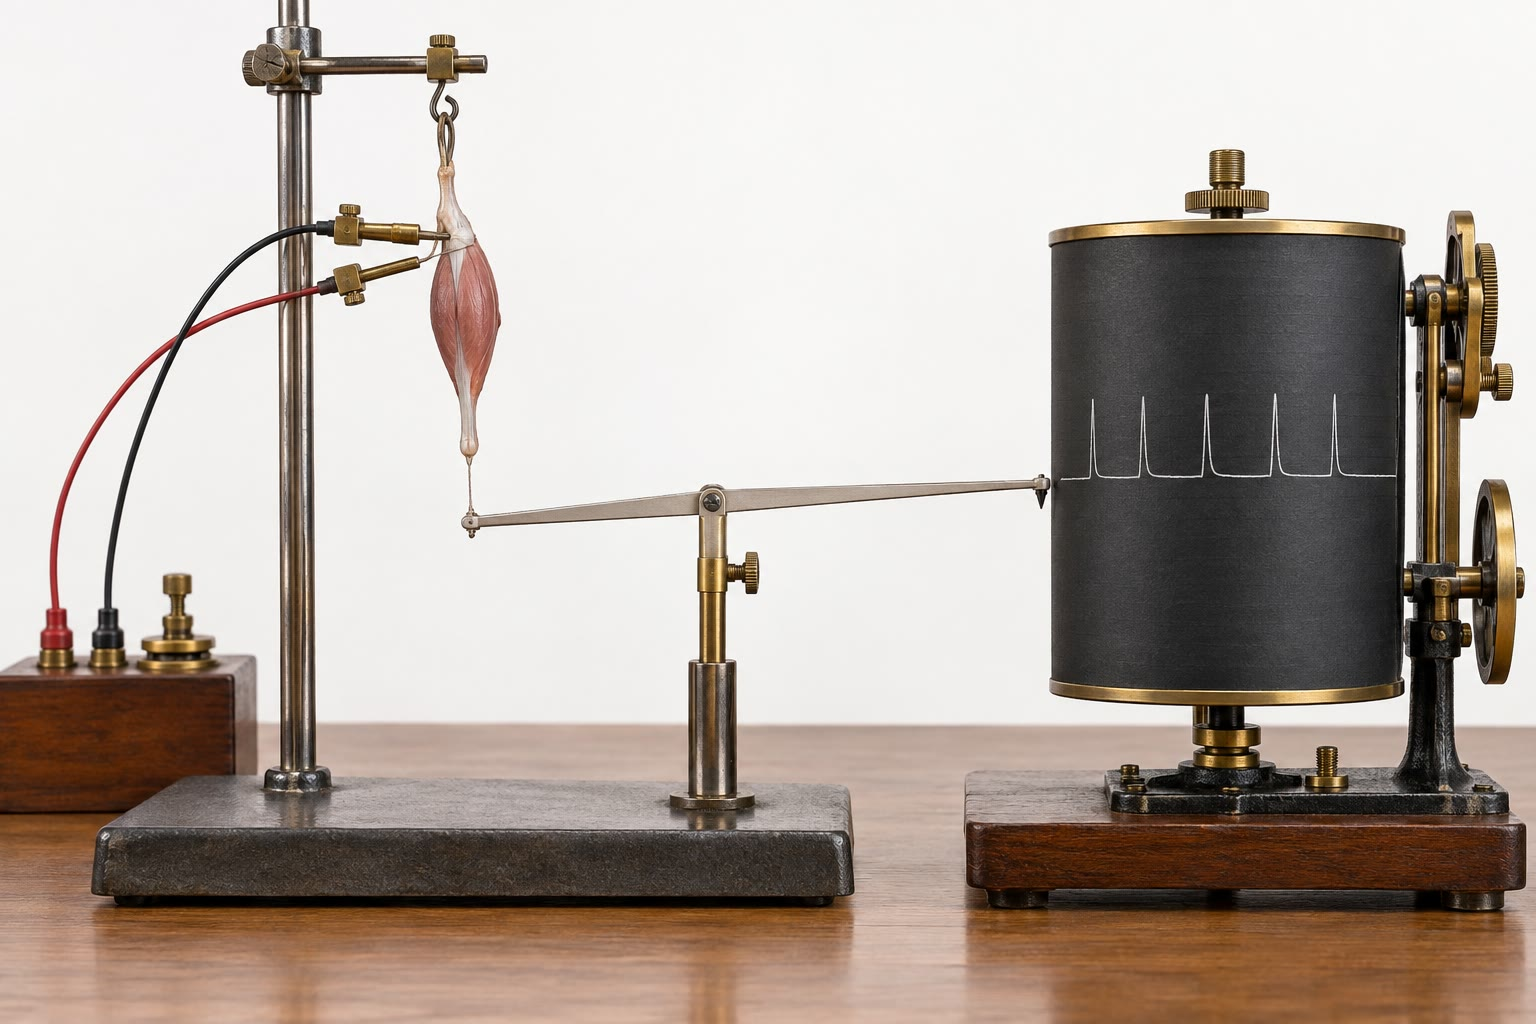
\includegraphics[width=0.44\linewidth]{images/book4/ai/b4-21-frog-muscle-prep.jpg}\hspace{0.04\linewidth}
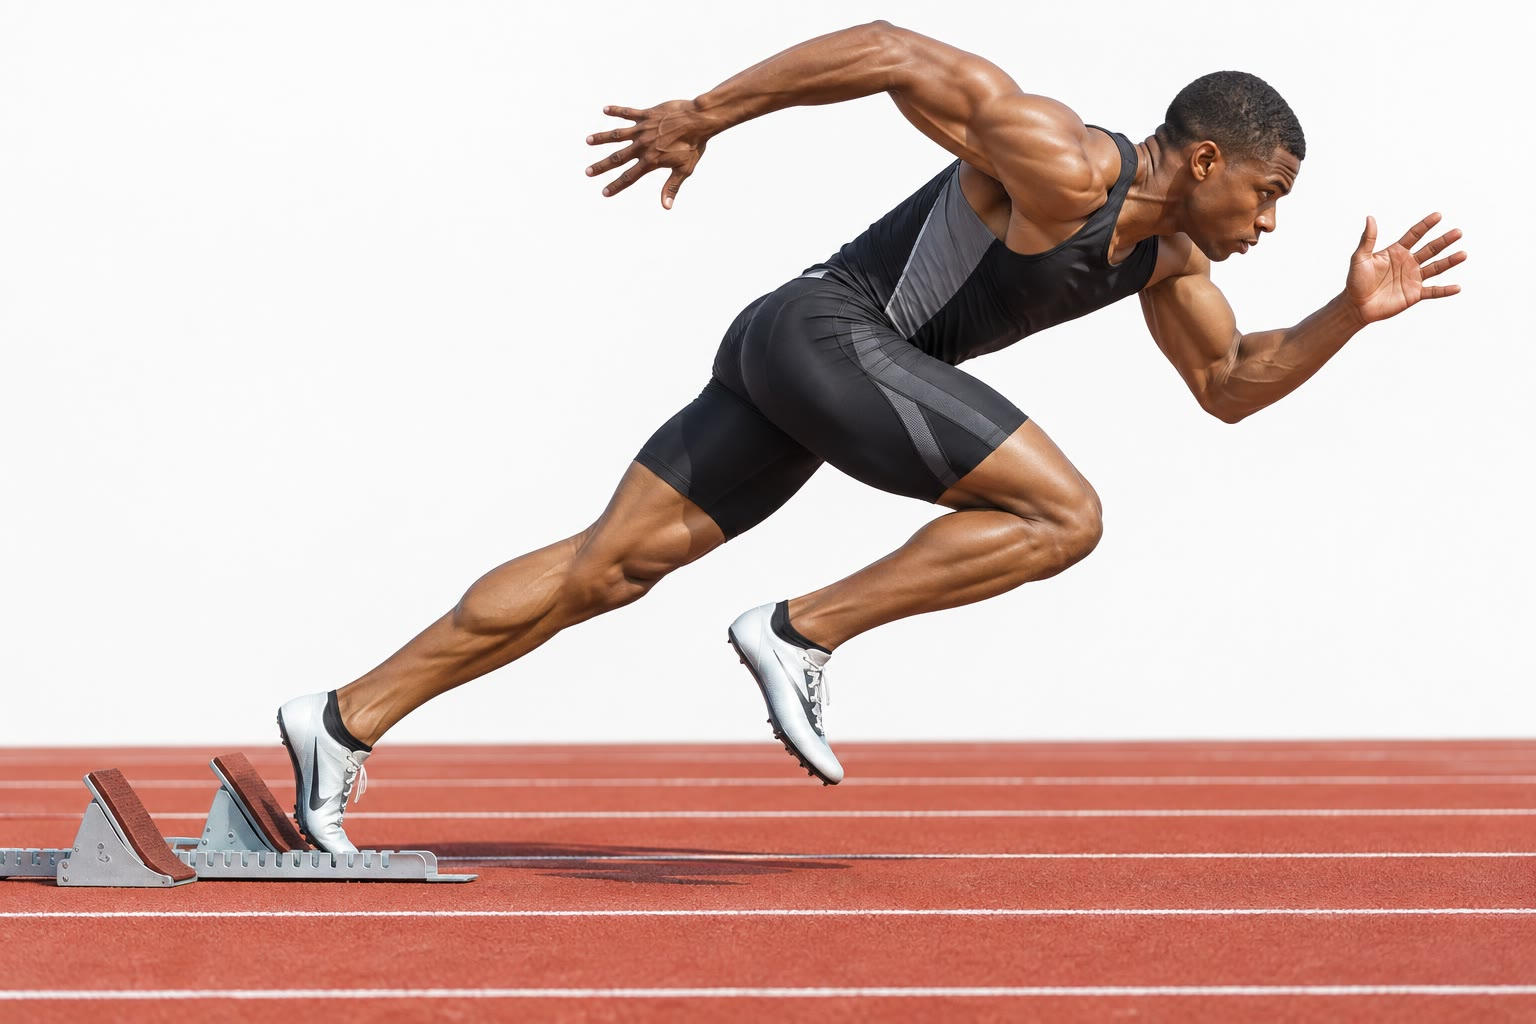
\includegraphics[width=0.44\linewidth]{images/book4/ai/b4-21-sprinter.jpg}

{\small Links: het klassieke preparaat --- een kikkerspier, haar zenuw,
prikkelelektroden en een hefboom die op een beroete trommel schrijft ---
waarop \omterm{def:b2:muscle-movement:motorunit}{enkelvoudige contractie}, summatie en \omterm{def:b2:muscle-movement:motorunit}{tetanus} voor het eerst werden
geregistreerd. Rechts: dezelfde fysiologie op volle kracht.}
\end{omfigure}

\section{Brandstof en vermoeidheid}

\begin{proposition}[Het werk betalen]\label{prop:b2:muscle-movement:energy}
\index{creatinefosfaat}\index{spiervermoeidheid}\index{zuurstofschuld}
Een vezel bevat ATP voor een seconde of twee volle inspanning. De eerste
reserve is \emph{\omterm{prop:b2:muscle-movement:energy}{creatinefosfaat}}, dat ADP binnen milliseconden opnieuw
fosforyleert en zo'n tien seconden meegaat --- de brandstof van de sprinter.
De tweede is de \emph{glycolyse} van het glycogeen van de vezel, zonder
zuurstof, die twee ATP per glucose en lactaat oplevert: snel, genoeg voor een
minuut of twee, en zelfbeperkend doordat zuur en fosfaat zich ophopen. De
derde is het \emph{oxidatieve} metabolisme van glucose en vetzuren in de
mitochondriën, dertig ATP per glucose, alleen beperkt door de zuurstof die het
\omterm{def:b2:blood-circulation:blood}{bloed} aanvoert (\cref{ch:b2:blood-pressure}): de marathon. Snelle glycolytische
vezels steunen op de eerste twee en raken in een minuut vermoeid; trage
oxidatieve vezels, rood van myoglobine en vol mitochondriën, houden het uren
vol. \emph{Vermoeidheid} bij een korte inspanning is niet de uitputting van
ATP --- die de spier in rigor zou achterlaten --- maar de ophoping van fosfaat
en protonen, die de dwarsbruggen en de calciumafgifte verzwakken; bij een
lange inspanning is het de uitputting van glycogeen en, uiteindelijk, van de
wil. Na de inspanning betaalt de spier haar \emph{\omterm{prop:b2:muscle-movement:energy}{zuurstofschuld}} terug: ze
herstelt het \omterm{prop:b2:muscle-movement:energy}{creatinefosfaat}, zet het lactaat weer om (in de lever) en vult
haar voorraden aan, en ademt nog minutenlang zwaar nadat ze stilstaat.
\end{proposition}

\begin{example}[Honderd meter]\label{ex:b2:muscle-movement:sprint}
Tien seconden maximale inspanning door \qty{20}{kg} beenspier met
\qty{100}{W/kg} is \qty{2}{kW} mechanisch vermogen en, bij een rendement van
\qty{25}{\%}, \qty{8}{kW} aan ATP-omzet --- zo'n \qty{160}{mmol} ATP per
seconde, of \qty{800}{g} ATP tijdens de race. De spier bevat enkele tientallen
grammen; \omterm{prop:b2:muscle-movement:energy}{creatinefosfaat} levert de eerste vijf seconden, glycolyse de rest,
en de sprintster finisht met lactaat op \qty{15}{mmol/L} in haar \omterm{def:b2:blood-circulation:blood}{bloed} en een
schuld die ze in het volgende kwartier afbetaalt. Een marathonloopster die
twee uur lang \qty{300}{W} levert, verbruikt \qty{2}{MJ} arbeid, \qty{8}{MJ}
brandstof --- een kilogram glycogeen en vet --- met zuurstof die de hele weg
met \qty{4}{L/min} wordt aangevoerd, en de muur waar ze bij de dertigste
kilometer tegenaan loopt, is de bodem van haar glycogeen.
\end{example}

\section{Opgaven}

\begin{exercise}[$\star$]\label{exo:b2:muscle-movement:1}
Formuleer het mechanisme van de \omterm{prop:b2:muscle-movement:sliding}{glijdende filamenten} en zeg welke banden van
het \omterm{def:b2:cell-differentiation:fibre}{sarcomeer} bij contractie veranderen en welke niet.
\end{exercise}

\begin{exercise}[$\star$]\label{exo:b2:muscle-movement:2}
Geef de vier stappen van de \omterm{prop:b2:muscle-movement:crossbridge}{dwarsbruggencyclus} en de rol van ATP in elke stap.
Waarom wordt een spier zonder ATP stijf?
\end{exercise}

\begin{exercise}[$\star$]\label{exo:b2:muscle-movement:3}
Noem de gebeurtenissen van een impuls in de motorische zenuw tot de hechting
van de myosinekoppen, met de tijd die elke gebeurtenis kost.
\end{exercise}

\begin{exercise}[$\star$]\label{exo:b2:muscle-movement:4}
Definieer \omterm{def:b2:muscle-movement:motorunit}{motorische eenheid}, \omterm{def:b2:muscle-movement:motorunit}{enkelvoudige contractie} en \omterm{def:b2:muscle-movement:motorunit}{tetanus}, en geef de
twee manieren waarop het zenuwstelsel kracht doseert.
\end{exercise}

\begin{exercise}[$\star\star$]\label{exo:b2:muscle-movement:5}
Een \omterm{def:b2:cell-differentiation:fibre}{sarcomeer} van \qty{2.4}{\micro m} verkort in \qty{50}{ms} tot
\qty{2.0}{\micro m}. Bereken de glijsnelheid van de dunne filamenten ten
opzichte van de dikke en, met een stap van \qty{10}{nm}, het aantal cycli dat
elke gebonden kop per seconde moet doorlopen.
\end{exercise}

\begin{exercise}[$\star\star$]\label{exo:b2:muscle-movement:6}
Een vezel van \qty{10}{cm} heeft \num{40000} sarcomeren in serie en verkort
met \qty{20}{\%} in \qty{0.1}{s}. Bereken haar verkortingssnelheid in lengtes
per seconde en in meter per seconde, en de snelheid van elk \omterm{def:b2:cell-differentiation:fibre}{sarcomeer}.
\end{exercise}

\begin{exercise}[$\star\star$]\label{exo:b2:muscle-movement:7}
Bereken met de relatie van Hill en $a = F_0/4$, $v_{\max} = 10$ lengtes per
seconde de kracht (als fractie van $F_0$) bij 1, 3 en 6 lengtes per seconde,
en het vermogen bij elke snelheid. Waar is het vermogen het grootst?
\end{exercise}

\begin{exercise}[$\star\star$]\label{exo:b2:muscle-movement:8}
Een quadriceps met een doorsnede van \qty{80}{cm^2} en \qty{30}{N/cm^2}:
bereken zijn maximale isometrische kracht. Hij grijpt \qty{5}{cm} van het
kniegewricht aan op een hefboom waarvan de voet \qty{45}{cm} van het gewricht
ligt: welke kracht kan de voet uitoefenen?
\end{exercise}

\begin{exercise}[$\star\star$]\label{exo:b2:muscle-movement:9}
De calciumpuls van een \omterm{def:b2:muscle-movement:motorunit}{enkelvoudige contractie} duurt \qty{30}{ms}. Leg uit
waarom impulsen met \qty{10}{Hz} een golvende kracht geven, met \qty{50}{Hz}
een gladde \omterm{def:b2:muscle-movement:motorunit}{tetanus}, en waarom de tetanische kracht de \omterm{def:b2:muscle-movement:motorunit}{enkelvoudige
contractie} overtreft.
\end{exercise}

\begin{exercise}[$\star\star\star$]\label{exo:b2:muscle-movement:10}
De \qty{20}{kg} beenspier van een sprinter levert \qty{10}{s} lang
\qty{2}{kW} bij een rendement van \qty{25}{\%}. Bereken het verbruikte ATP
(\qty{50}{kJ/mol}), het \omterm{prop:b2:muscle-movement:energy}{creatinefosfaat} dat nodig is voor de eerste
\qty{5}{s}, en de glucose die wordt gefermenteerd voor de rest (2 ATP per
glucose). Welke lactaatconcentratie geeft dat in \qty{40}{L} lichaamswater?
\end{exercise}

\begin{exercise}[$\star\star\star$]\label{exo:b2:muscle-movement:11}
Voorspel het effect op de contractie van: een middel dat het
calciumafgiftekanaal van het reticulum blokkeert; een middel dat de pomp
ervan blokkeert; een \omterm{def:b2:genome-diversification:mutation}{mutatie} die troponine ongevoelig maakt voor calcium; het
verwijderen van calcium uit het \omterm{def:b2:blood-circulation:blood}{bloed}, voor skeletspier en voor het \omterm{def:b2:heart:anatomy}{hart}.
\end{exercise}

\begin{exercise}[$\star\star\star$]\label{exo:b2:muscle-movement:12}
``Een spier is een machine die chemische energie omzet in kracht, met het
rendement van een goede motor en de sturing van een computer.'' Bespreek het
rendement (een kwart tot de helft), wat het beperkt, en wat de twee manieren
van het zenuwstelsel om kracht te doseren opleveren dat een enkele schakelaar
niet zou geven.
\end{exercise}

\section{Vraagstuk: de fysiologie van een sprong}

\begin{problem}[{Weekendvraagstuk --- een sprong uit stand geanalyseerd van
het sarcomeer tot de afzet: het glijden, de dwarsbruggen, de
calciumschakelaar, de kracht-snelheidsgrens, de motorische eenheden en de
brandstof, met als besluit het aantal slagen van de dwarsbruggen, de kracht
bij de afzetsnelheid en het ATP dat de sprong kost}]
\label{pb:b2:muscle-movement:1}
Iemand van \qty{70}{kg} springt \qty{40}{cm} recht omhoog en brengt het
massamiddelpunt van het lichaam \qty{0.4}{m} omhoog tijdens een afzet van
\qty{0.3}{s}. De strekspieren van de benen (\qty{20}{kg} spier) hebben samen
een doorsnede van \qty{500}{cm^2} met \qty{30}{N/cm^2}; hun vezels zijn
\qty{12}{cm} lang (\num{48000} sarcomeren) en verkorten tijdens de afzet met
\qty{4}{cm}; de gewrichten vermenigvuldigen de verkorting van de spier aan de
voet met \num{10} en delen haar kracht door dezelfde factor. $v_{\max} = 8$
lengtes per seconde, $a = F_0/4$. Elk dik filament draagt \num{300}
myosinekoppen; er zijn $6\times
10^{10}$ dikke filamenten per vierkante centimeter spier; een slag
is \qty{10}{nm} en kost één ATP (\qty{8e-20}{J}, \qty{50}{kJ/mol});
rendement \qty{40}{\%}. De spier bevat \qty{5}{mmol/kg} ATP en
\qty{20}{mmol/kg} \omterm{prop:b2:muscle-movement:energy}{creatinefosfaat}. De vezels zijn \qty{60}{\micro
m} dik. Motorische eenheden: \num{800} per spiergroep, met elk \num{50} tot
\num{2000} vezels.

\medskip
\noindent\textbf{Deel I --- De mechanica.}
\begin{enumerate}
  \item Bereken de afzetsnelheid die nodig is om \qty{40}{cm} te stijgen
        ($v^{2} = 2gh$), en de kinetische energie bij de afzet.
  \item Bereken de gemiddelde kracht die de benen tijdens de afzet op de
        grond uitoefenen (de arbeid over \qty{0.4}{m} is gelijk aan de
        kinetische energie plus de arbeid tegen de zwaartekracht), en
        vergelijk met het gewicht.
  \item Bereken de maximale isometrische kracht van de strekspieren en, met
        de hefboomverhouding van 10, de maximale kracht aan de voet die ze
        zou kunnen geven.
  \item Bereken de verkortingssnelheid van de vezels in lengtes per seconde
        en als fractie van $v_{\max}$.
  \item Bereken met de relatie van Hill de kracht die bij die snelheid
        beschikbaar is als fractie van $F_0$, en de kracht aan de voet die
        ze geeft. Kan de spier alleen de sprong maken? Waar komt de rest
        vandaan?
  \item Bereken het gemiddelde mechanische vermogen tijdens de afzet en het
        vermogen per kilogram strekspier.
\end{enumerate}

\medskip
\noindent\textbf{Deel II --- De dwarsbruggen.}
\begin{enumerate}[resume]
  \item Hoeveel verkort elk \omterm{def:b2:cell-differentiation:fibre}{sarcomeer}, en hoeveel slagen van
        \qty{10}{nm} moeten er langs elk half \omterm{def:b2:cell-differentiation:fibre}{sarcomeer} worden gemaakt om de
        filamenten zover te laten glijden?
  \item Bereken de glijsnelheid in elk half \omterm{def:b2:cell-differentiation:fibre}{sarcomeer} en het aantal slagen per
        seconde dat een kop zou maken als hij voortdurend gebonden was.
  \item Bereken het aantal myosinekoppen in de strekspieren.
  \item Bereken de arbeid die de spier zelf levert (haar kracht bij de
        snelheid van de sprong maal haar verkorting), de arbeid per slag bij
        een rendement van \qty{40}{\%}, en het aantal benodigde slagen.
  \item Hoeveel slagen per kop is dat, tegenover het aantal dat volgens
        vraag 7 beschikbaar is? Geef commentaar op de reserve.
  \item Bereken het ATP dat de sprong verbruikt, in mol en in gram
        (\qty{507}{g/mol}), en controleer het rendement met de energie van
        dat ATP.
\end{enumerate}

\medskip
\noindent\textbf{Deel III --- De schakelaar en het bevel.}
\begin{enumerate}[resume]
  \item De afzet duurt \qty{0.3}{s} en de calciumpuls van één impuls
        \qty{30}{ms}. Welke vuurfrequentie houdt de vezels in \omterm{def:b2:muscle-movement:motorunit}{tetanus}, en
        hoeveel impulsen stuurt elk motorisch \omterm{def:b2:neurons-synapses:neuron}{neuron}?
  \item Het vrije calcium stijgt van \qty{0.1}{} tot \qty{10}{\micro
        mol/L} in een vezel van \qty{5e-10}{L}. Hoeveel vrije calciumionen
        zijn dat, en hoeveel pompcycli (twee ionen per ATP) kost het om ze
        terug te halen?
  \item Bereken het aantal vezels in de strekspieren en het ATP van de
        dwarsbruggen per vezel per impuls, en vergelijk met de pompkosten van
        vraag 14. De werkelijke kosten van het pompen bedragen ongeveer een
        kwart van het ATP van de spier: wat onderschat het vrije calcium?
  \item Het zenuwstelsel rekruteert eenheden naar grootte. Welke eenheden
        worden voor de sprong gerekruteerd, en in welke volgorde? Welke
        fractie van de \num{800} zou een rustige stap gebruiken?
  \item Leg uit waarom de kracht bij een lage inspanning fijn en dicht bij het
        maximum alleen grof kan worden gedoseerd.
  \item Iemand gebruikt een middel dat de \omterm{prop:b2:neurons-synapses:integration}{neuromusculaire overgang} voor de
        helft blokkeert: voorspel de \omterm{def:b2:muscle-movement:motorunit}{enkelvoudige contractie}, de \omterm{def:b2:muscle-movement:motorunit}{tetanus} en
        de sprong.
\end{enumerate}

\medskip
\noindent\textbf{Deel IV --- De brandstof.}
\begin{enumerate}[resume]
  \item Bereken het ATP dat in de strekspieren is opgeslagen en vergelijk
        met het verbruik van de sprong.
  \item Bereken de voorraad \omterm{prop:b2:muscle-movement:energy}{creatinefosfaat} en het aantal sprongen dat die
        zou kunnen betalen.
  \item Tien sprongen na elkaar: welke brandstof neemt het over, en wat
        hoopt zich op?
  \item Het \omterm{def:b2:blood-circulation:blood}{bloed} kan de strekspieren \qty{2}{L} zuurstof per minuut leveren
        (6 ATP per $\mathrm{O_2}$). Welke ATP-omzet vraagt het vermogen van de
        sprong, en welke zuurstoftoevoer zou dat vergen? Trek een conclusie.
  \item Na de sprongen ademt de persoon een minuut lang zwaar. Bereken de
        zuurstof die nodig is om het verbruikte \omterm{prop:b2:muscle-movement:energy}{creatinefosfaat} en ATP opnieuw
        te synthetiseren (\qty{6}{ATP} per $\mathrm{O_2}$-molecuul) en
        vergelijk met het rustverbruik van \qty{250}{mL/min}.
  \item Waarom gaat de spier van een springer niet in rigor, ook al wordt ATP
        in zo'n tempo omgezet?
  \item Formuleer het resultaat: de slagen per half \omterm{def:b2:cell-differentiation:fibre}{sarcomeer}, de
        krachtfractie bij de snelheid van de sprong, en het ATP dat de sprong
        kost.
\end{enumerate}
\end{problem}
